\documentclass[crop,tikz]{standalone}

\begin{document}

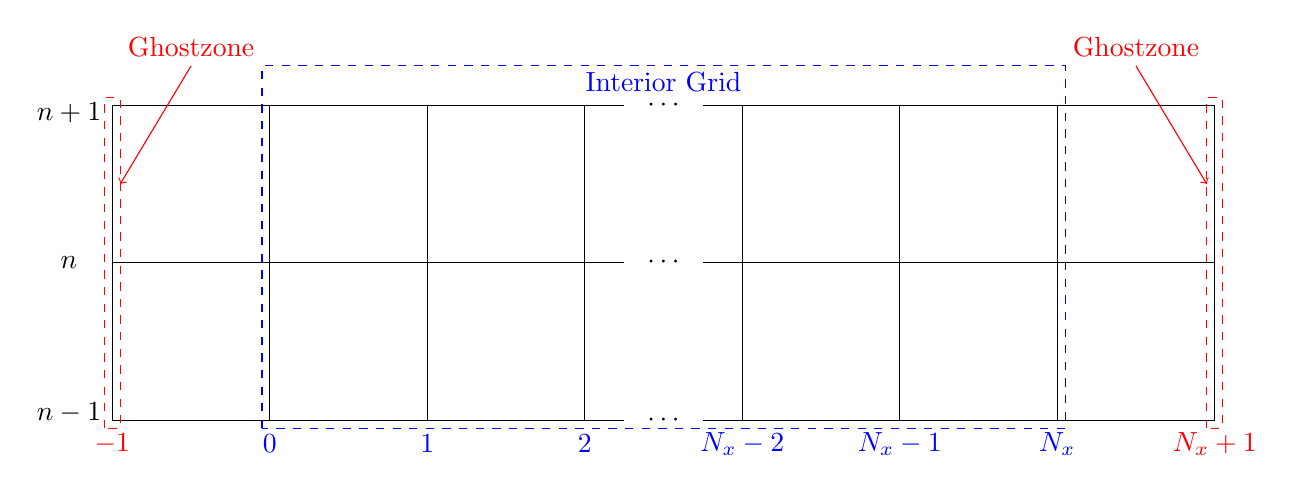
\begin{tikzpicture}
  \node (x0) at (0,-0.3) {$\color{red}-1$};
  \node (x1) at (2,-0.3) {$\color{blue}0$};
  \node (x2) at (4,-0.3) {$\color{blue}1$};
  \node (x3) at (6,-0.3) {$\color{blue}2$};
  \node (x4) at (8,-0.3) {$\color{blue}N_{x}-2$};
  \node (x5) at (10,-0.3) {$\color{blue}N_{x}-1$};
  \node (x6) at (12,-0.3) {$\color{blue}N_{x}$};
  \node (x7) at (14,-0.3) {$\color{red}N_{x}+1$};
  \node (y0) at (-0.55,0.1) {$n-1$};
  \node (y1) at (-0.55,2) {$n$};
  \node (y2) at (-0.55,3.9) {$n+1$};
  \node (d0) at (7,0) {$\cdots$};
  \node (d1) at (7,2) {$\cdots$};
  \node (d2) at (7,4) {$\cdots$};
  \node (d3) at (7,4.3) {\color{blue}{Interior Grid}};
  \draw (0,0) grid[xstep=2,ystep=2] (6,4);
  \draw (6,0) -- (6.5,0);
  \draw (6,2) -- (6.5,2);
  \draw (6,4) -- (6.5,4);
  \draw (7.5,0) -- (8,0);
  \draw (7.5,2) -- (8,2);
  \draw (7.5,4) -- (8,4);
  \draw (8,0) grid[xstep=2,ystep=2] (14,4);
  \draw[color=blue,dashed] (1.9,-0.1) rectangle (12.1,4.5);
  
  \draw[color=red,dashed] (-0.1,-0.1) rectangle (0.1,4.1);
  \draw[<-,color=red] (0.1,3) -- (1,4.5) node[above] {Ghostzone};
  
  \draw[color=red,dashed] (13.9,-0.1) rectangle (14.1,4.1);
  \draw[<-,color=red] (13.9,3) -- (13,4.5) node[above] {Ghostzone};
\end{tikzpicture}

\end{document}